\section{Processus de reconfiguration} 

\begin{frame}{Processus de conception de reconfiguration existant}
\begin{figure}
\begin{subfigure}[b]{0.45\textwidth} % "0.45" donne ici la largeur
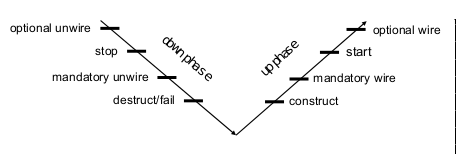
\includegraphics[width=5cm, height=3.8cm]{imgs/boyer_protocole}
\caption{Automatique, \emph{Boyer et al, 2017}}\label{fig:orchid}
\end{subfigure}
\begin{subfigure}[b]{0.45\textwidth} % "0.45" donne ici la largeur
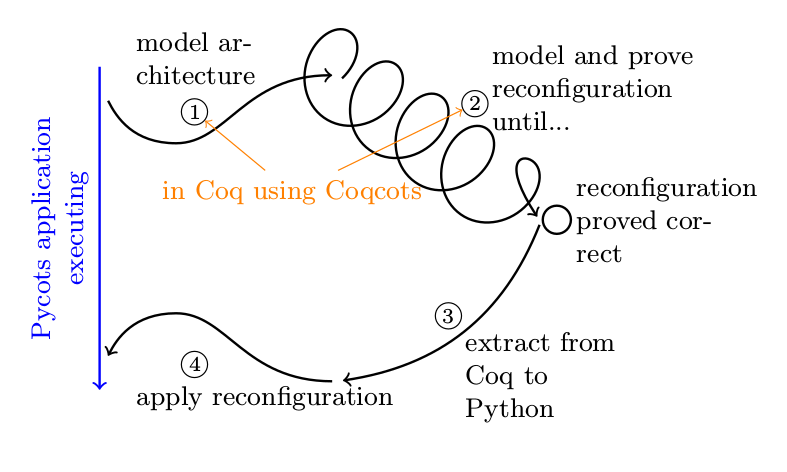
\includegraphics[width=5cm]{imgs/buisson_approche}\\
\caption{Manuelle \emph{Buisson et al, 2017}}\label{fig:orchid}
\end{subfigure}
\end{figure}
\end{frame}

\begin{frame}{Proposition d'un processus de reconfiguration}
\begin{figure}
\centering
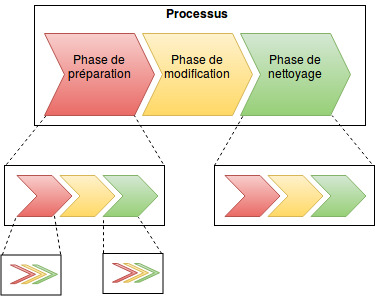
\includegraphics[width=8cm]{imgs/phases-de-reconfiguration.jpg}
\end{figure}
\end{frame}

\begin{frame}{Utilisation des patrons de reconfiguration}
Le processus s'appuie sur les patrons de reconfiguration. Dans un
premier temps, l'architecte analyse les modifications à apporter.\\

il utilise le catalogue de patron pour identifier les problèmes qu'il
peut rencontrer et comment les résoudre. ou il définit un nouveau
patron. \\

Dans le cas, ou le solution n'est pas directement applicable alors il
peut décider d'une nouvelle itération .
\end{frame}
